% General beamer options %
%%%%%%%%%%%%%%%%%%%%%%%%%%

%\documentclass[handout]{beamer} % activar esta para imprimir handouts, desactivar la de abajo, y desactivar shownotes (sin overlays)

\documentclass[]{beamer} % para presentaciones

% Class options include: notes, notesonly, handout, trans,
%                        hidesubsections, shadesubsections,
%                        inrow, blue, red, grey, brown

%\usepackage{pgfpages} %This is needed for notes presentation con dual monitor
%\setbeameroption{show notes on second screen=left} % para presentaciones con dual monitor
%\setbeameroption{show notes}  % muestra notas de presentacion intercaladas a las slides
%\setbeameroption{show only notes} % crea documento solo con notas
\setbeamerfont{note page}{size=\tiny} % achica tamaño letra notas (default: small)

% Theme for beamer presentation.
\usepackage{beamerthemesplit} 

	% para cambiar el color del theme
	\definecolor{mycolor}{RGB}{100,100,100} % para definir color personalizado, luego reemplazar abajo (ej bg=mycolor) 
	\setbeamercolor*{palette primary}{use=structure,fg=white,bg=mycolor}


% Other themes include: beamerthemebars, beamerthemelined, 
%                       beamerthemetree, beamerthemetreebars  


\setbeamercovered{transparent} % esto hace que las transiciones entre items sean transparentes

%\setbeamertemplate{footline}[frame number] % for inserting page numbers, but in this theme eliminates the whole footer (!)

% This is a macro for inserting page numbers without eliminating the footer

\newcommand*\oldmacro{}%
\let\oldmacro\insertshorttitle%
\renewcommand*\insertshorttitle{%
  \oldmacro\hfill%
  \insertframenumber\,/\,\inserttotalframenumber}
\usepackage{graphicx}

% Other latex useful options
%---------------------------

%\usepackage{mathtools}   % loads »amsmath« , for equations
\usepackage{textgreek} % para poder escribir caracteres griegos en el texto sin pasar a mathmode
\usepackage[utf8]{inputenc}  % permite escribir acentos directamente. PERO: asegurarse que en caso de colaboración el colaborador tenga opción utf8 predeterminada en su editor de LATEX ... si no, no funciona
\usepackage{booktabs}% tablas
\usepackage{outlines} % permite mayor flexibilidad en algunas listas


% Define information for the title page %
%%%%%%%%%%%%%%%%%%%%%%%%%%%%%%%%%%%%%%%%%

\usepackage{textpos}

\title[Sociología de la Educación 2016 - SOL 141] % this is the reduced title for the foots
{\textsc{\large{Ciudadanía y participación}}}

%\subtitle{Proyecto doctoral}

\author[Daniel Miranda] % this is the reduced author for the foot
{{{\small Daniel Miranda \textsuperscript{1}}}}

\institute{\textsuperscript{1}
	Pontificia Universidad Católica de Chile \\
	Facultad de Ciencias Sociales \\ 
	Instituto de Sociología \\  
	%	COES FONDAP/CONICYT/15130009 \\ 
	%	CONICYT-PCHA/Doctorado Nacional/2015 \\ 
	
	%\vspace{5mm} Committe: \\
	%Prof. Juan Carlos Castillo (Advisor)\\
	%Prof. Matías Bargsted \\
	%Prof. Cristian Cox
	}

\date {\begin{tiny}
		{Septiembre 21, 2016} %, for today date
	\end{tiny}}
	% Enter the date or \today between curly braces

% BEGIN PRESENTATION %
%%%%%%%%%%%%%%%%%%%%%%
\begin{document} % Creates title page of slide show using above information

\begin{frame}[plain,label=firstframe] % plain is for removing the bars from the top & the bottom in this title slide
  \titlepage
\end{frame}
\note[itemize]{
\item X
} 

%\section[Outline]{}  % removed because I did not wanted it to be in the sections menu at the top
% Creates table of contents slide incorporating all \section and \subsection commands

%\begin{frame}
%	\frametitle{Contents}
%  \tableofcontents
%\end{frame}

\begin{frame}
	\frametitle{Contenidos}
	\tableofcontents
\end{frame}

\section{Democracia, ciudadanía y escuela} 

\begin{frame} [allowframebreaks]
	%\frametitle{Could sociological theory illuminate the youth citizen's involvement?}
	\begin{itemize}
		\item  “..las monocracias, las autocracias, las dictaduras son fáciles, nos caen encima solas; las democracias son difíciles, tienen que ser promovidas y creídas” (Sartori, 1991, p.118).
	\end{itemize}
\end{frame}
	
	
\subsection{Rol de la escuela}
	
\begin{frame}	
	\begin{itemize}
		\item Socialización política: Entender el proceso por medio del cuál las personas de encuentran su lugar en el sistema político es (y han sido) un tema de preocupación (Tockeville; Niemi \& Hepburn, 1995; Greenstein, 1965; Hyman, 1969; Langton, 1969; Abendschon, 2013; Ekman \& Amna, 2014) 
		
		\item Supuesto: Lo que se aprende en edades tempranas tiende a permanencer: persistencia de la socializaciión (Hooghe, 2004)
		
		\item Agentes de socialización: Familia, escuela, pares, medios, instituciones.
		
		\item La escuela...
		
	\end{itemize}
\end{frame}

\begin{frame}
	Los sistemas escolares nacen atados a dos ideales normativos (Peña, 2014)
	\begin{itemize}
		\item Meritocracia: escuela como ecualizador de las condiciones de origen social
		
		\item Ciudadanía: separación de la incondicionalidad del hogar, permitiría la adquisicion de virtudes y valores necesarios para la vida democrática.
		
		\item \textbf{¿Puede la escuela fortalecer esos ideales?}
		
	\end{itemize}
\end{frame}

	
\section{Formación Ciudadana en Chile}

\subsection{Antecedentes}

\begin{frame} [allowframebreaks]
	
	\begin{figure}
		\centering
		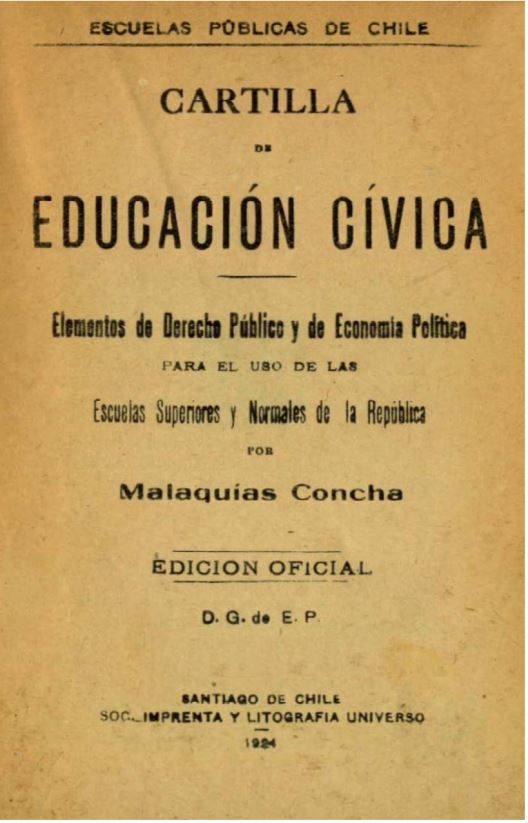
\includegraphics[width=0.4\linewidth]{p1}
		%\caption{IDEA, 2016}
	\end{figure}
	
	\begin{itemize}
		\item "La \textbf{educación cívica debe constituir una de las principales materias del programa escolar}. La democracia gana terreno en el mundo entero. La libertad y la igualdad se establecen así en las Monarquías como en las Repúblicas...

	\framebreak
		\item ...\textbf{Si los ciudadanos no saben distinguir las reglas más elementales} de justicia, de buena administración y de previsión que un país debe observar en interés de su conservación y prosperidad; si se imaginan mejorar su suerte por medio de la expoliación o la violencia, entonces el gobierno popular no haría otra cosa que cavar la tumba a la libertad.
		
	\framebreak
		\item \textbf{El sufragio es el pedestal del gobierno democrático}; es menester esforzarse en interés de las instituciones es republicanas, por esparcir la capacidad política en la inteligencia de la instrucción cívica, sólida y general debe siempre preceder al sufragio universal" (p.1).
	\end{itemize}
\end{frame}

\begin{frame} [allowframebreaks]

	El curriculum de Educación Ciudadana, Desde el 80 hasta ahora, ha sido redefinido 4 veces (Cox \& García, 2014)
		\begin{itemize}
					\item 1980-1981: Centrado en la familia y valores nacionalistas.
					\item Con un curso de educación Cívica en los dos últimos años, con foco en constitución y democracia portegida.
				\framebreak
					\item 1996 para Básica y 1998 en Media: Reorganiza la formación en diversas asignaturas.
					\item Historia y ciencias sociales, orientación, Filosofía y Psicología.
				\framebreak
					\item Ajuste curricular 2009: Enfásis e contenidos como: Intitucionalidad política y compromiso ciudadano.
					\item Se mantiene distribuido.
				
				\framebreak
					\item Ajuste curricular 2013: se explicita eje de formación ciudadana:
					\item En Historia, geografía y ciencas sociales desde 1ro básico a 2do Medio.
		\end{itemize}
\end{frame}

\subsection{Plan de Formación Ciudadana 2016}
\begin{frame} [allowframebreaks]
	
	\begin{figure}
		\centering
		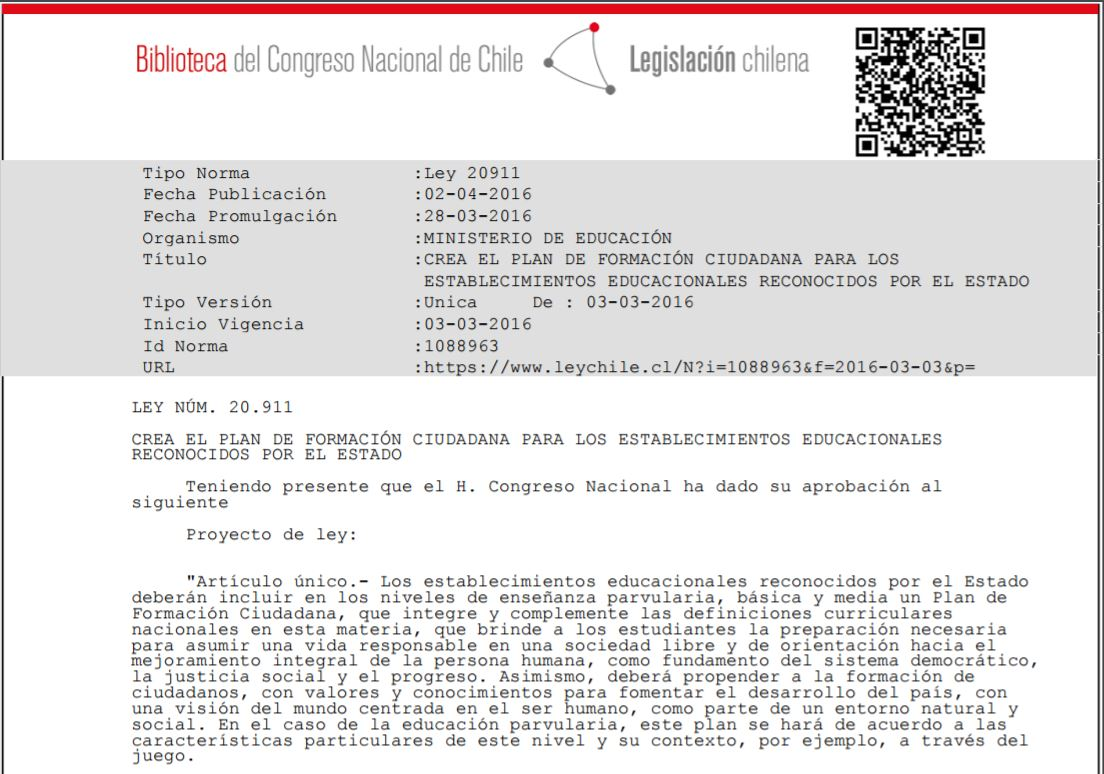
\includegraphics[width=0.9\linewidth]{plan}
		%\caption{Van Deth, 2001}
	\end{figure}
	
	\begin{itemize}
		\item La ley Nº 20.911 dispone que todos los establecimientos educacionales reconocidos por el Estado deberán incluir en los niveles educativos que impartan –parvularia, básica y/o media— un Plan de Formación Ciudadana, que integre y complemente las definiciones curriculares nacionales para brindar a las y los estudiantes la preparación necesaria en este ámbito.
		
		\item El Ministerio de Educación propone que este Plan se articule con el Proyecto Educativo Institucional (PEI) y con el Plan de Mejoramiento Educativo (PME).
		
		\item Se espera que el plan brinde a los estudiantes la preparación necesaria para asumir una vida responsable en una sociedad libre y de orientación hacia el mejoramiento integral de la persona humana, como fundamento del sistema democrático, la justicia social y el progreso. Asimismo, deberá propender a la formación de ciudadanos, con valores y conocimientos para fomentar el desarrollo del país, con
		una visión del mundo centrada en el ser humano, como parte de un entorno natural y social.
	\end{itemize}
\end{frame}

\begin{frame} [allowframebreaks]
	\frametitle{Objetivos del Plan}
	\begin{itemize}
		\item Promover la \textbf{comprensión y análisis del concepto de ciudadanía} y los derechos y deberes asociados a ella, entendidos éstos en el marco de una República democrática, con el propósito de formar una \textbf{ciudadanía activa} en el ejercicio y cumplimiento de estos derechos y deberes.
		\item Fomentar en las y los estudiantes el ejercicio de una ciudadanía crítica, responsable, respetuosa, abierta y creativa.
		\item Promover el conocimiento, comprensión y análisis del Estado de Derecho y de la institucionalidad local, regional y nacional, y la formación de virtudes cívicas en el estudiantado.
	
	\framebreak
		\item Promover el conocimiento, comprensión y compromiso de los y las estudiantes con los derechos humanos reconocidos en la Constitución Política de la República y en los tratados internacionales suscritos y ratificados por Chile, con especial énfasis en los derechos del niño.
		\item Fomentar en los y las estudiantes la valoración de la diversidad social y cultural del país.
		\item Fomentar la participación del estudiantado en temas de interés público.
	
	\framebreak
		\item Garantizar el desarrollo de una cultura democrática y ética en la escuela.
		\item Fomentar una cultura de la transparencia y la probidad.
		\item Fomentar en los estudiantes la tolerancia y el pluralismo.
	\break

		\textbf{¿Qué modelo de ciudadano y democracia contiene el plan?}
	\end{itemize}
\end{frame}	
	
\section{Modelo(s) de democracia}

\begin{frame} [allowframebreaks]
	\begin{itemize}
		\item Democracia liberal
			\begin{itemize}
				\item Mínima (voto)
				\item Sistema de partidos (número razonable)
				\item Ciudadanos autonomos con habilidades y conocimientos básicos
				\item Coformidad con reglas y procedimientos
			\end{itemize}
		
		\item Republicanismo cívico
			\begin{itemize}
				\item Ciudadanos activos
				\item Activismo político
				\item Altos niveles de conocimientos y habilidades
				\item Crítica en el nombre del bien común
			\end{itemize}
			
	\framebreak
		\item Democracia crítica
			\begin{itemize}
				\item Creando justicia social
				\item Activismo social y político
				\item Crítica y mejora de la igualdad a travez de la acción polítia y social
				\item En retirada luego de las crisis
			\end{itemize}
		\item Democracia cosmopolita 
			\begin{itemize}
				\item Más allá de límites nacionales (global)
				\item Interés en los problemas del mundo
				\item Celebración de la diversidad
			\end{itemize}
		
	
	\end{itemize}
\end{frame}

\section{Modelo(s) de ciudadanía}
\subsection{¿Crisis o nuevas ciudadanías?}

\begin{frame} [allowframebreaks]

	\begin{itemize}
\item Participación: Cambio (proliferación) de los repertorios de participación (Van deth, 2001)
		
			\begin{figure}
				\centering
				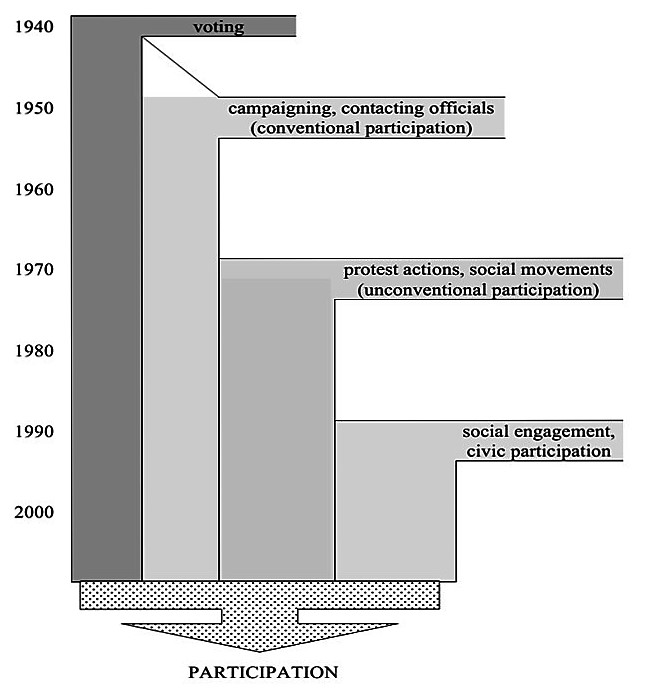
\includegraphics[width=0.6\linewidth]{Vandeth}
				%\caption{Van Deth, 2001}
			\end{figure}
			
	\framebreak
	
		\item Paradoja de la participación, sobre todo en cohortes más jóvenes
				
		\item Disminución de la participación en voto como amenaza a la representatividad de los sistemas democráticos (Blais \& Rubenson, 2013).
		
			\begin{figure}
				\centering
				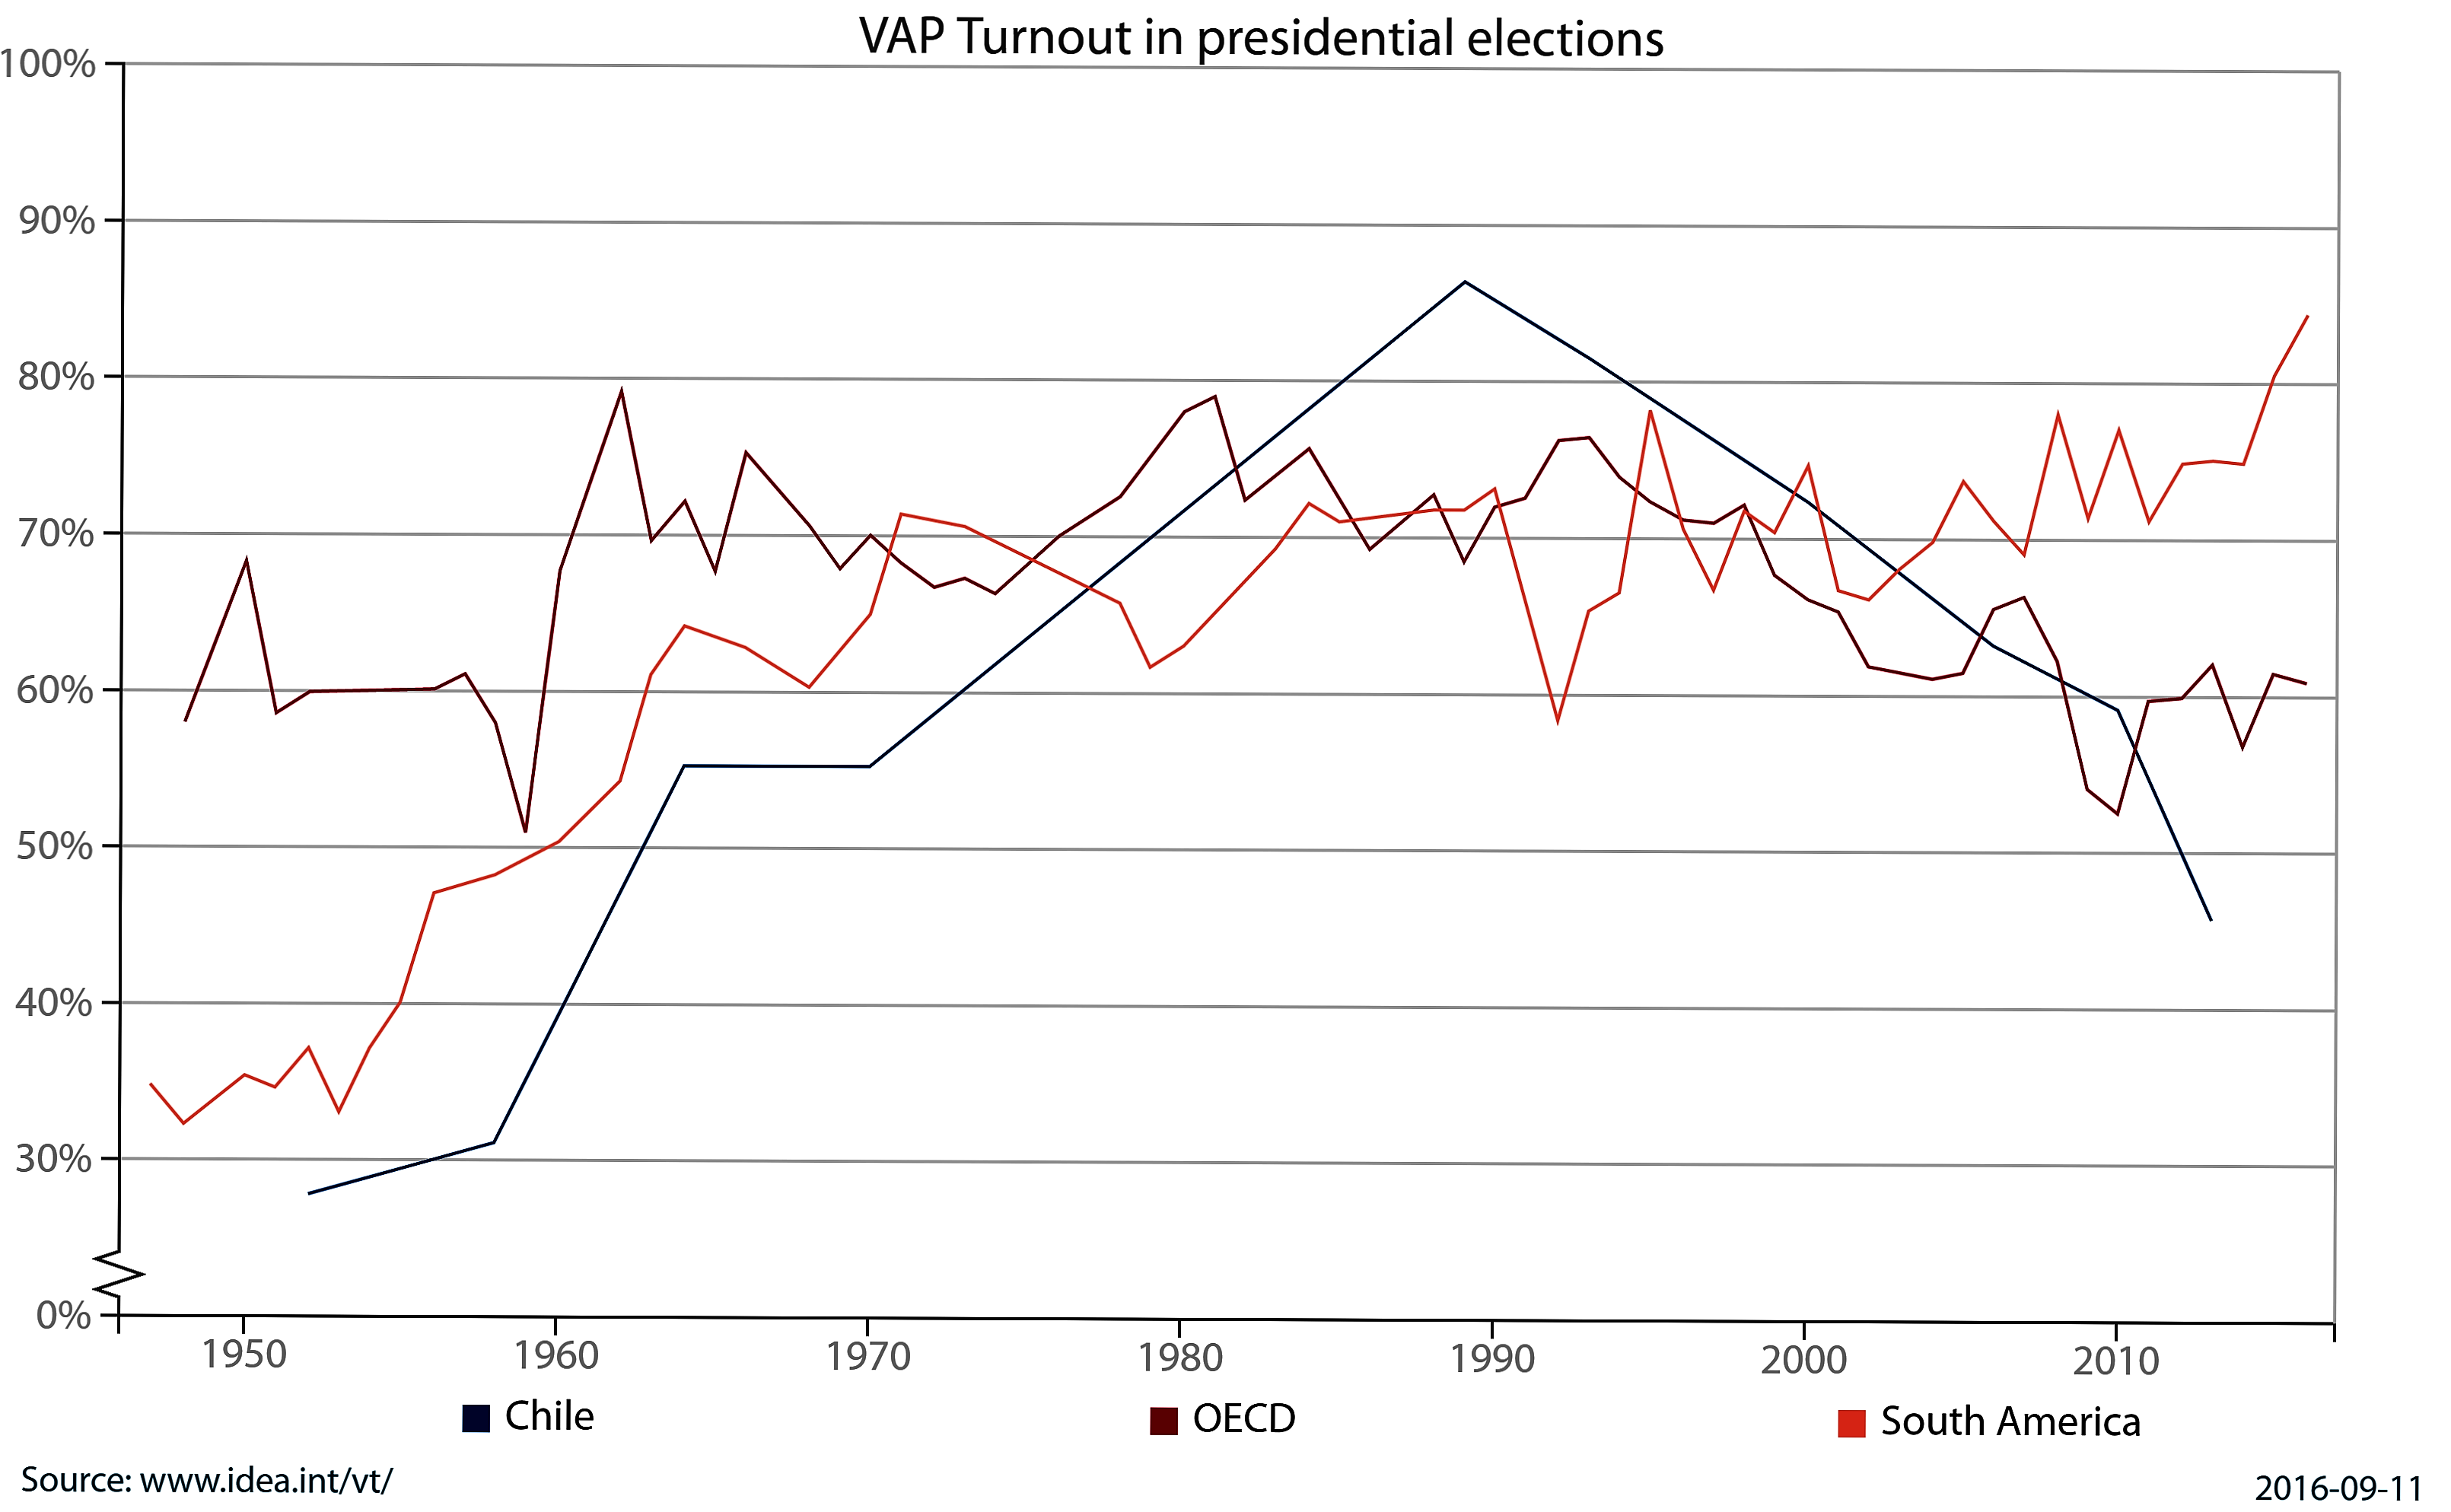
\includegraphics[width=0.8\linewidth]{VAP}
				%\caption{IDEA, 2016}
			\end{figure}
			
			
		\framebreak
		
		\item Desigualad política: otra amenaza.
		\begin{itemize}
			\item Desigualdad Social y su relación con desigualdad política
			\item Aumento de las desigualdes sociales (Picketty, 2014; GINI project, 2012). 
			\item Los efectos de los sesgo socieconómicos se observan desde edades tempranas, indicando desigualdad política desde el inicio (Verba, Burns \& Schlozman, 2003; 2015)
			\item Estos sesgos socioeconómicos serían una amenaza importante a los ideales democráticos de igualdad en la participación y representación.
			
		\end{itemize}
		
	\framebreak
		\item Sin embargo, al considerar otras formas de participación los patrones sugieren que las cohortes jóvenes prefieren canales alternativos (o no institucionales) de participación (García-Albacete, 2014).
	\framebreak	
			\begin{figure}
				\centering
				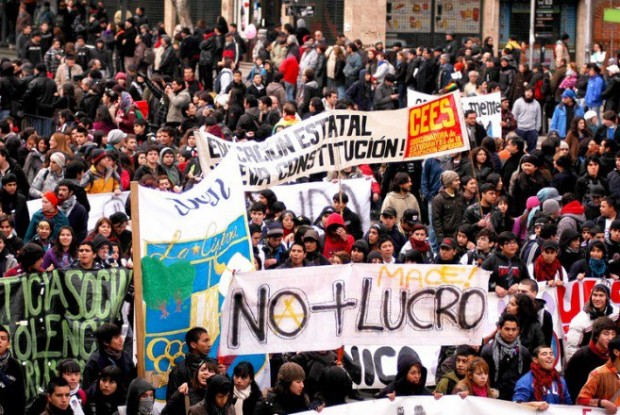
\includegraphics[width=0.7\linewidth]{lucro}
				%\caption{IDEA, 2016}
			\end{figure}
			
				\begin{figure}
					\centering
					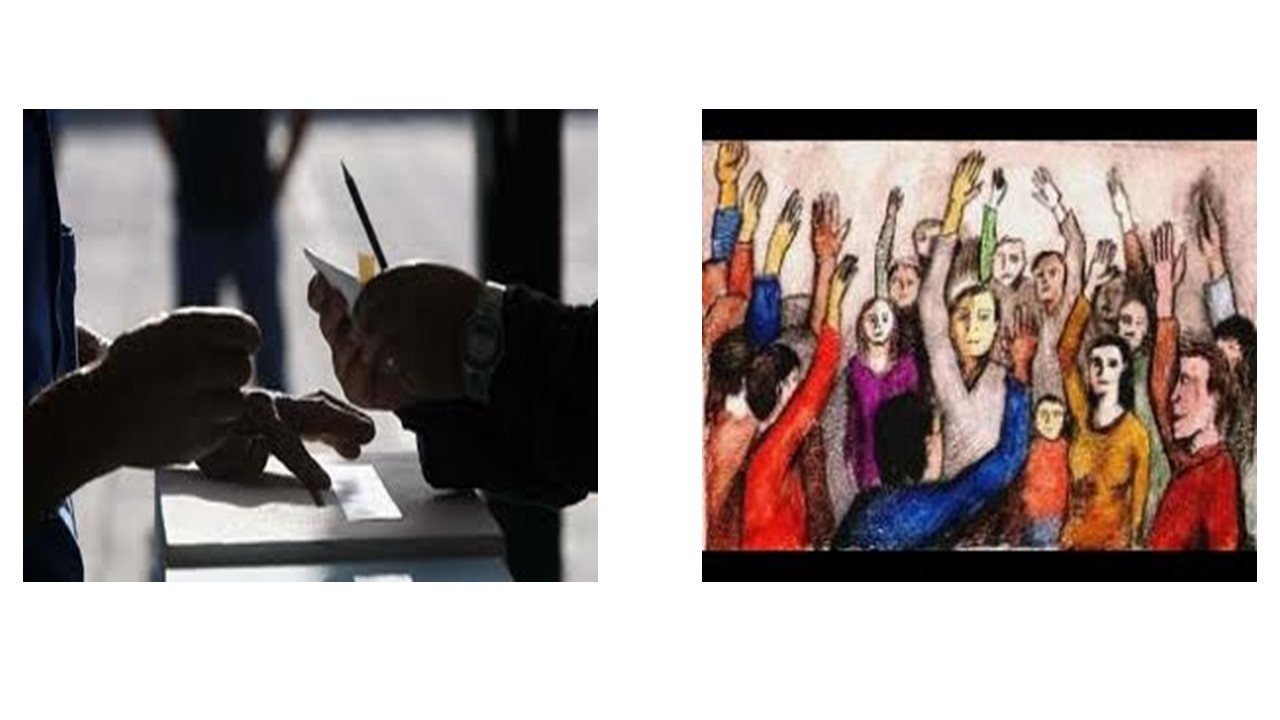
\includegraphics[width=0.7\linewidth]{civciv_foto}
					%\caption{IDEA, 2016}
				\end{figure}
		
		\item Por tanto, capturar las diversas formas de participción parece adecuado para abordar la participación juvenil.
					
		\item Considerando que en población juvenil la pregunta por la participación se convierte en una pregunta acerca del funcionamiento futuro de la democracia (Van Deth, 2011).
		
		\item Sin embargo, votar y las manifestaciones públicas no son suficientes para cubrir todos los aspectos necesarios.
		
			\begin{itemize}
				\item ¿Qué queda por cubrir?
			\end{itemize}
			
		\end{itemize}
	\end{frame}	
			
\subsection{Modelos posibles}
\begin{frame} [allowframebreaks]
	\begin{itemize}
	\item "participation in civil society, community and/or political life, characterized by mutual respect and non-violence and in accordance with human rights and democracy” (2006¸ pp. 4). 
	
				\begin{itemize}
					\item Sociedad civil
					\item Comunidad
					\item Vida política
					\item Respeto mutuo
					\item no violencia
					\item derechos humanos
					\item democracia
				\end{itemize}
	
		\begin{figure}
			\centering
			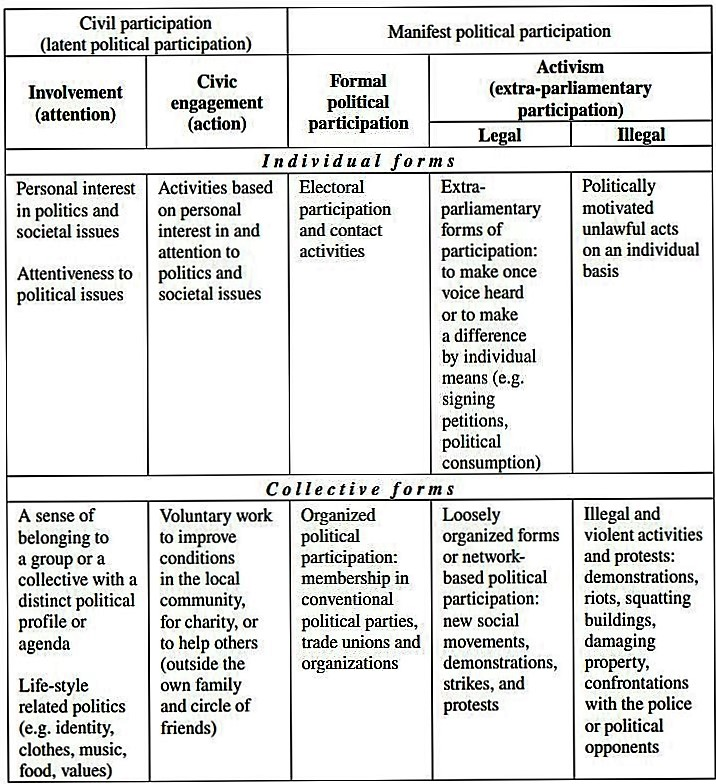
\includegraphics[width=0.6\linewidth]{ekmanamna}
			%\caption{IDEA, 2016}
		\end{figure}
		
	\framebreak
		\begin{figure}
			\centering
			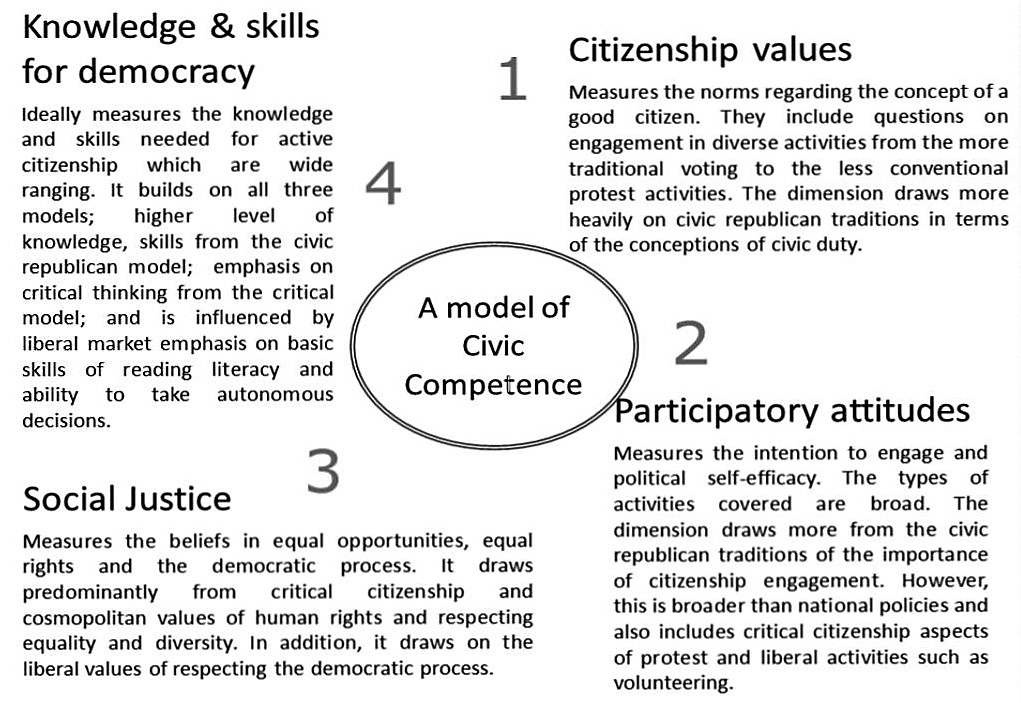
\includegraphics[width=0.6\linewidth]{Hmodel}
			%\caption{IDEA, 2016}
		\end{figure}
		
	\framebreak
	\begin{figure}
		\centering
		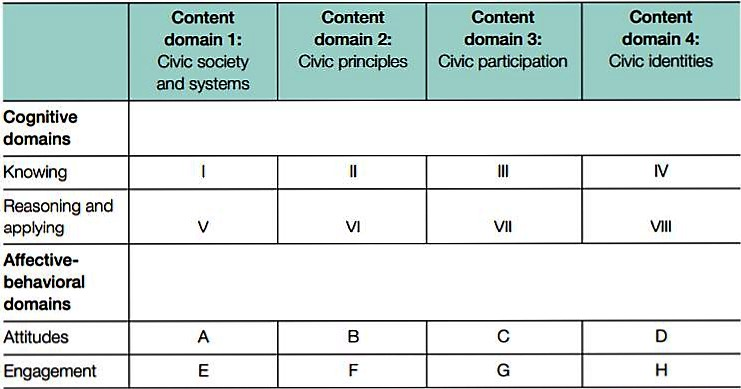
\includegraphics[width=0.8\linewidth]{ICCS2016}
		%\caption{IDEA, 2016}
	\end{figure}
	
	\framebreak
	\begin{figure}
		\centering
		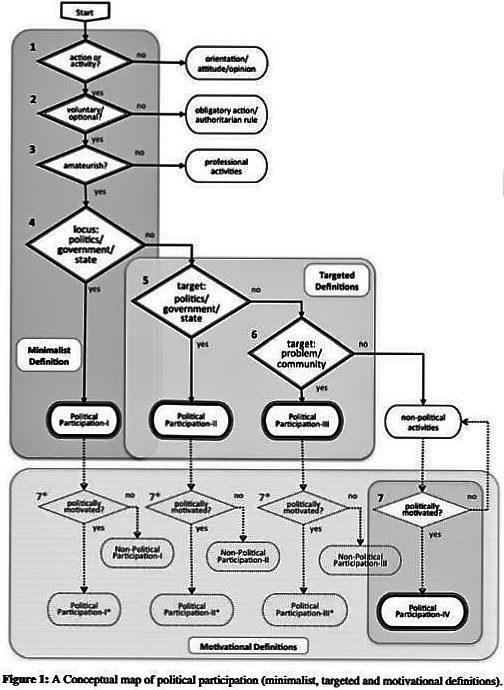
\includegraphics[width=0.6\linewidth]{mapdeth}
		%\caption{IDEA, 2016}
	\end{figure}
	\end{itemize}
\end{frame}

\section{Estudios Nacionales e Internacionales}

\begin{frame} [allowframebreaks]
	\begin{itemize}
		\item \textbf{IEA Civic Education Study, CIVED 1999}. Australia, Belgium (French), Bulgaria, Canada, \textbf{Chile}, Colombia, Cyprus, Czech Republic, Denmark, England, Estonia, Finland, Germany, Greece, Hong Kong SAR, Hungary, Israel, Italy, Latvia, Lithuania, Netherlands, Norway, Poland, Portugal, Romania, Russian Federation, Slovak Republic, Slovenia, Sweden, Switzerland, and United States.
		
	\framebreak
		\item \textbf{International Civic and Citizenship Education Study, ICCS 2009}
		
		\begin{figure}
			\centering
			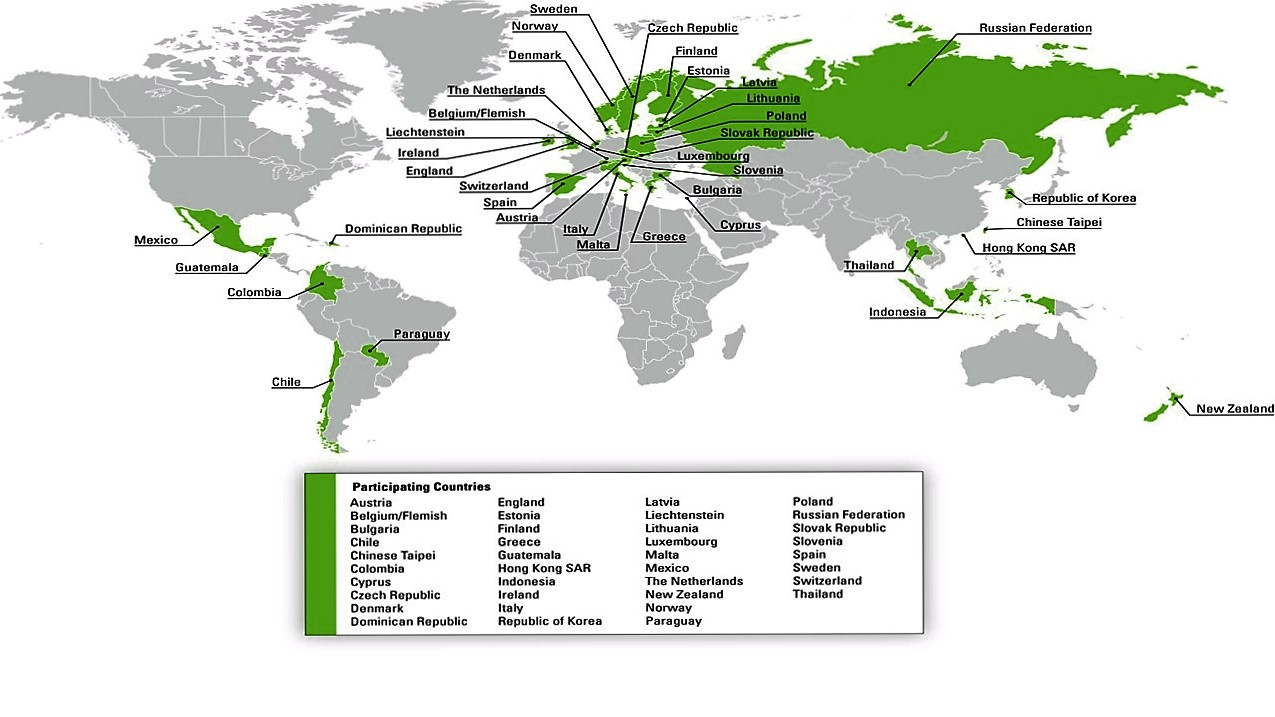
\includegraphics[width=1\linewidth]{sample}
			%\caption{Van Deth, 2001}
		\end{figure}
		
		\item \textbf{International Civic and Citizenship Education Study, ICCS 2016}: Belgium (Flemish), Bulgaria,\textbf{Chile}, Chinese Taipei, Colombia, Croatia, Denmark, Dominican Republic, Estonia, Finland, Germany (North Rhine-Westphalia), Hong Kong SAR, Italy, Korea, Latvia, Lithuania, Malta, Mexico, Netherlands, Norway, Peru, Russian Federation, Slovenia, and Sweden.
		
		
		\item CELS: The Citizenship Educational Longitudinal Study - 2001-2010 \url{https://www.nfer.ac.uk/research/projects/cels/}
		
		\item Estudio Panel Sueco. Desde 2009: 5000 adolescentes y adultos jóvenes entre 13-30 por un periodo de 6 años.
		\url{https://www.oru.se/PSP/}
		
		\item Belgian Political Panel Survey (BPPS), 2006-2011. 6000 adolescentes.\\ \url{https://lirias.kuleuven.be/handle/123456789/314889}
		
			\begin{figure}
				\centering
				\includegraphics[width=1\linewidth]{libro}
				\label{fig:Vandeth}
				%\caption{Van Deth, 2001}
			\end{figure}
	\end{itemize}
\end{frame}
	
	
%========================================================
\againframe[plain]{firstframe} % repite slide inicial

\end {document}

 % Basic frame
 
	\begin{frame}%[allowframebreaks]{Outline} 
	\frametitle{XX} 
  	\begin{itemize}%[<+->] % este signo al lado del itemize es para las transiciones entre items
  	\item 
  	\item 
    \end{itemize}    
	\end{frame}
	
	\note [itemize]{
	\item I
	} 

<1-> : después de \item permite ordenar el orden de aparición según el número 

% Insertar figuras
  	\begin{figure}[h]
	\begin{centering}
	\includegraphics [scale=0.1]{simon}
	\end{centering}
	\end{figure} 
	
		
% Figuras a la derecha del texto

    \begin{columns}
    	\column{0.30\linewidth}
        \centering
        \includegraphics[scale=0.35]{aqui imagen}
        \column{0.70 \linewidth}
		\textbf{titulo del texto a la derecha}
		\begin{itemize}
			\item XX  
	\end{itemize}			              
    \end{columns} 
    
% weblinks
\href{https://www.statmodel.com}{\beamergotobutton{www}}


	\begin{frame}[allowframebreaks] % [fragile] 
		\frametitle{Variables} 
		\textbf{Reported civil participation} (1. No, I have never done this 2.Yes, I have done this but more than a year ago
		3.Yes, I have done this within the last twelve months)
		\begin{itemize}
			\item Environmental organization
			\item Human rights organization
			\item A voluntary group doing something to help the community
			
		\end{itemize}
		
		\textbf{Reported civic participation}
		\begin{itemize}
			\item Taking part in decision making about how the school is run
			\item Taking part in discussions at a student assembly
			\item Becoming a candidate for class representative or school parliament
		\end{itemize}
		
		\framebreak
		
		\textbf{Intended civil participation} (1: I will certainly not do this 4.	I will certainly do this ) \\
		\begin{itemize}
			\item Write to a newspaper about political and social issues
			\item Contribute to an online discussion forum about social and political issues
			\item Join an organization for a political or social cause
		\end{itemize}
		
		\textbf{Intended civic participation} 
		\begin{itemize}
			\item Vote in local elections
			\item Vote in national elections
			\item Get information about candidates before voting in an election
		\end{itemize}
		\framebreak
		\textbf{Independent variables} 
		\begin{itemize}
			\item individual variables (Political interest, ethnic background, gender)
			\item family indicators (parent’s education level, Occupation prestige Index ISEI, Class Index EGP proxy, Books at home)
			\item School’s indicators characteristics (Administrative dependency, socioeconomic level, Citizenship practices) 
			\item Country level indicators (GDP, Inequality Index, Democracy index, Civil Society index)
		\end{itemize}
	\end{frame}

\subsection{Results}

\begin{frame}%[allowframebreaks] % [fragile] 
	\frametitle{Confirmatory Factor Analysis} 
	\begin{figure}[h]
		\begin{centering}
			\includegraphics [scale=0.30]{CCCFA}
		\end{centering}
	\end{figure}
	
	$\chi^2=794.04$, df=48, $p<0.001$, CFI=0.989, RMSEA=0,023.
\end{frame}

\begin{frame}%[allowframebreaks] % [fragile] 
	\frametitle{Invariance} 
	\begin{scriptsize}
		\begin{table}[H]
			\centering
			\caption{Measurement invariance of civic-civil model of citizenship}
			\begin{tabular}{rrrrrrrr}
				\hline
				& \textbf{Chi-square} & \textbf{df} & \textbf{P value} & \textbf{CFI} & \textbf{RMSEA} & \textbf{diff CFI} & \textbf{diff RMSEA} \\
				\hline
				Configural & 1055,11 & 288   & 0     & 0,992 & 0,023 &       &  \\
				Metric & 1404,55 & 328   & 0     & 0,989 & 0,026 & 0,003 & 0,003 \\
				Scalar & 1782,14 & 398   & 0     & 0,986 & 0,027 & 0,003 & 0,001 \\
				\hline
			\end{tabular}%
			\label{tab:addlabel}%
		\end{table}%
	\end{scriptsize}
\end{frame}

\begin{frame}[allowframebreaks] % [fragile] 
	\frametitle{Descriptives} 
	\begin{figure}[h]
		\begin{centering}
			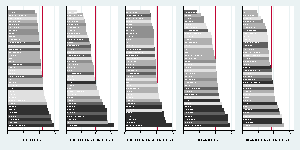
\includegraphics [scale=0.6]{between}
		\end{centering}
	\end{figure} 	
	\framebreak
	\begin{figure}[h]
		\begin{centering}
			\includegraphics [scale=0.6]{whitin}
		\end{centering}
	\end{figure}    
\end{frame}

\subsection*{}

\begin{frame}%[allowframebreaks] % [fragile] 
	\frametitle{Discussion} 
	\begin{itemize}%[<+->] % para transiciones entre items
		\item Confirmatory evidence for the civic-civil model of citizenship participation 
		\item Model tested at scalar invariant level 
		\item Country comparison reveal different levels in the participation dimension
		\item Predominance of the civil orientation of citizenship, particularly in Guatemala, Dominican Republic and Colombia. 
		\item Invariance allows future studies based on the measurement model as dependent / independent variables	
	\end{itemize}    
\end{frame}      


\begin{frame}[allowframebreaks] % [fragile] 
	\frametitle{Problem and relevance} 
	\begin{itemize}%[<+->] % para transiciones entre items
		\item Several ways of understanding citizenship:
		\begin{itemize}
			\item From "thin" citizenship, oriented to vote as the main way to participate in the public life (\textbf{civic dimensions})
			\item To "thick" or wider concepts of citizenship, based on values of equality and human rights that considers citizens as agents of social change in different contexts and/or groups (\textbf{civil dimensions})
			\item Also, Civil Society it is considered crucial in order to maintain a minimum level of civic virtue (Van Deth, 2001)
		\end{itemize}  
	\end{itemize}	
\end{frame}]	



	\framebreak		
	\item Contextual effects (Country)
	\begin{itemize}
		\item The influence of country context on civic attitudes has been a fundamental topic of interest since the beginning of the comparative research projects on civic issues (Kerr, 2012; Kerr, 2015).
		\item Evidence shows that country context as development, religious composition, democratic system or years of democracy can influence the rates of participation in civil associations. 
		\item Some evidence shows that the political inequalities are accentuated in societies with greater exposure to inequality (Lancee \& Van de Werfhorst, 2011),
	\end{itemize}

